\chapter{Introduction to Messaging} 

This chapter will at first provide a basic introduction to messaging and will
uncover the fallacies of messaging, which will lead to the need for a
Message-Oriented-Middleware. The primary focus is set on a detailed analysis of a
message broker system, which is related to the broker pattern. During this
chapter, other terms will be declared which will play an important role to
understand the capabilities of Apache Kafka.

\begin{figure}[H]
    \centering
    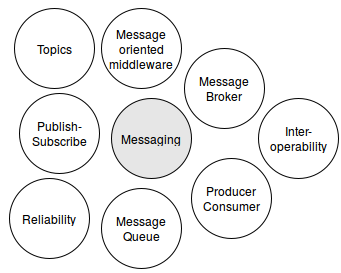
\includegraphics[width=0.3\textwidth]{images/messaging-intro.png}
    \caption{Messaging terms}
    \label{fig:MBig:the-log}
\end{figure}

\section{What is Messaging?}

A distributed system consists of a collection of multiple autonomous components,
connected through a network, which enables to coordinate  their activities (e.g.\
computers) and to share resources. To a user, these systems appear as a
single, integrated computing facility. Unlike centralised systems,
distributed systems have their advantages in economics, performance and
scalability and reliability. In fact, this approach allows to build reliable
applications, scaled using low cost computers, and thus can serve massive
performance needs whether on demand or continuously.  Although distributed
systems have many advantages, compared to local applications, they also bring
many challenges, as explained in detail later on, which have to be considered by 
developers.\cite{POSA1}\cite{TAN06}

\begin{figure}[H]
    \centering
    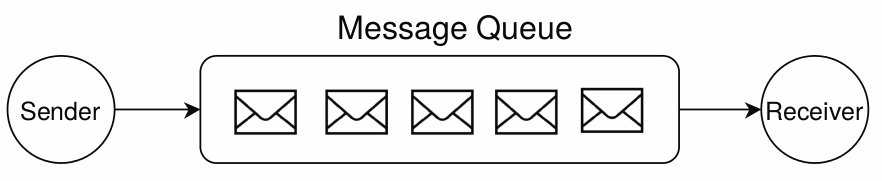
\includegraphics[width=0.5\textwidth]{images/messaging-simple.png}
    \caption{Basic principle of a message queue}
    \label{fig:messaging-simple}
\end{figure}

Messaging integrates distributed applications to an overall system by providing
message queues for communication between them (see figure
\ref{fig:messaging-simple}). One application can publish its messages to the
queue and another application can asynchronously read from it at any time.
A message is just a simple and independent unit with a data structure
which contains a meta header and the transmitted information. The messaging
technology enables high-speed, asynchronous, program-to-program communication
with reliable delivery.

\newpage
Peter Deutsch originally defined fundamental fallacies of distributed computing
which still are relevant today.\cite{fallaciesOfDs} Messaging
simplifies the development of distributed systems by mainly facing the
following:

\begin{enumerate}
    \item{\textbf{Fallacy: The network is reliable}

        There are always plenty of things that can go wrong in a network, like
        power failures, bad connectivity or natural disasters. Therefore a
        network must never be seen as fail-safe. One always has to assume that
        sent data is possibly getting lost on the wire. A messaging system runs
        with an underlying middleware (\ref{intro-messaging-mom}) which deals
        with failures on each side of the communication. This allows to get
        knowledge about which messages has been successfully delivered and which
        need to be redelivered. Thus, the original sender never has the guarantee
        that the sent message has arrived at the desired destination, but it
        always has the confirmation of the middleware that the data has been put 
        in a message queue. In case of failure the messaging system can initiate
        appropriate actions to delegate a failed transmission.

      }

    \item{\textbf{Fallacy: Bandwidth is infinite and the Latency is zero }

        Since communicating over network is significantly slower than local
        operations, a distributed system has to deal with delays and
        interruptions of any length. Messaging supports a storage capacity which
        leads to a persistent way of communication where it is not required that
        the collaborating endpoints are active during the entire transmission of
        a message. This loose coupling in time is achieved by working with
        queues as data structure (first-in-first-out).

      }

    \item{\textbf{Fallacy: Topology doesn't change}

        Applications, systems and topologies change over time, and in most
        scenarios this will often affect the collaborating components in the
        distributed network too. Therefore distributed nodes should be decoupled
        as far as possible. Messaging tries to achieved this with the underlying
        middleware.(\ref{intro-messaging-mom}) The sender and receiver do not need
        to know whether or not to communicate, nor do they need to know the other 
        side directly. They always communicate via the middleware software. In 
        case of significant changes, only the interface to the messaging system 
        needs to be updated.

      }

    \item{\textbf{Fallacy: The network is homogeneous}

        In the real world, applications are always different. In distributed systems
        data needs to be transmitted between nodes which use different
        programming languages, operating platforms, and data formats.  This is
        called interoperability which actually means that systems based on
        different technologies can collaborate together by using the same
        standards or protocols. Messaging provides either a common interface or
        a protocol on the wire which can be implemented by various
        applications. When using a messaging system in an enterprise
        environment, it is much more efficient to integrate a new application to
        the existing data flow instead of implementing a new interface for
        another technology. The newly introduced component can be linked to the
        existing platform by just using the underlying messaging protocol.\\

        In the past, several companies like IBM or Microsoft developed their own
        proprietary standards and protocols for asynchronous messaging systems
        -- probably to keep it locked in their customer base. In June 2001 the
        Java Message Service API (JMS) was released as the best-known standard for
        messaging systems. However, it is only an interface without a specific
        protocol, JMS implementations need to define their own. Fortunately in
        June 2006 a pool of multiple companies for network technologies defined
        the Advanced Message Queueing Protocol (AMQP) as an open standard for an
        interoperable messaging protocol. \cite{PrpAMQP}

    }

\end{enumerate} \cite{EIP03}\cite{fallacies}

\newpage

\section{Message Oriented Middleware}
\label{intro-messaging-mom}

Because networks are not inherently reliable, messaging would never be
efficient without a systems that manages the capabilities of messaging by acting
as mediator. To introduce an intermediate component between distributed
applications may be a very good choice as it would reduce the close coupling of
communication styles such as sockets-based or RMI/RPC. This additional component
is known as the messaging system or message-oriented middleware (MOM) and is
all about passing messages in any format from one application to another where
the parties do not need to knows each other directly. \cite{TAN06} The MOM
provides a specific API for both the sender and the receiver:

\begin{table}[H]
\centering
\begin{tabular}{|l|l|}
\hline
\textbf{Put}    & Append a message to a specific queue                                        \\ \hline
\textbf{Get}    & Block until the specific queue is nonempty, and remove the first message    \\ \hline
\textbf{Poll}   & Check a specific queue for messages, and remove the first                   \\ \hline
\textbf{Notify} & Install a handler to be called when a message is put into a specified queue \\ \hline
\end{tabular}
\caption{Basic API for message queue implementation \cite{TAN06}}
\end{table}

In a basic scenario including an application A being the sender of a message and
an application B being the receiver, the MOM -- running either on the node itself
or dedicated in the local network -- holds a local queue to store incoming
messages and manages an address-lookup database for mapping destination names to
network locations. Overall, the flow of a message sent from A to B will be as
follows: first, the sender packs its data into the appropriate message format
(1) and puts the message in a local queue (2). The MOM then delivers the message
over the network to the local queue of the receiver (3). Finally, the receiver
system fetches the message and stores it in its own local queue (4) to
further unpack and finally get the transmitted data (5).

\begin{figure}[H]
    \centering
    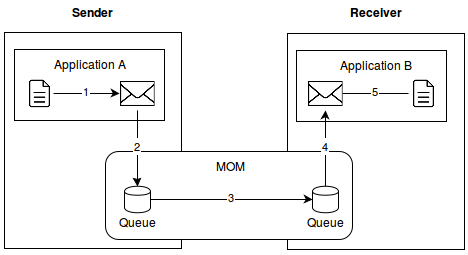
\includegraphics[width=0.5\textwidth]{images/mom-schema.png}
    \caption{Schematic flow of communication in a basic messaging system }
    \label{fig:message-oriented-middleware}
\end{figure}

\section{Topologies}
\subsection{Point-To-Point Connection}
\label{intro-messaging-pointtopoint}
A point-to-point connection is the simplest architecture for communicating in a
messaging system. It ensures that only one node receives a specific message by
setting up particular connections between the nodes. This kind of
communication works well in an environment with only a few systems which want to
collaborate and use the advantages of messaging. But if there are more
nodes, the local mapping of a queue name to a foreign network location
implies that each system needs to hold the addresses of all the other nodes that it
wants to communicate with. When a target address changes, all the applications that
communicate with the changed target must be updated. 

In most scenarios there is also a need for transforming messages to a different
format where these implementations have to be made on every node, which leads to
duplicating code. In an architecture with many collaborating applications,
point-to-point messaging can end up in a mesh, of connections which is hard to
maintain.  For more complex integration solutions, a centralised solution
whereas the MOM runs on a location-independent platform is required. This is
where the central hub (broker) comes into game. \cite{MSDNIntegration}

\begin{figure}[H]
    \centering
    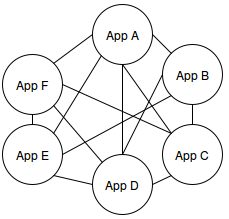
\includegraphics[width=0.35\textwidth]{images/point-to-point-messaging.png}
    \caption{Mesh of multiple point-to-point connections}
    \label{fig:point-to-point-messaging}
\end{figure}

\subsection{Central Hub (Message Broker)}
\label{intro-messaging-broker}
A messaging system with point-to-point connections can decouple two systems
by using a managed queue on each side of a collaboration. But there is
still the need of configuring the endpoints on each side. In general, a
message broker is a dedicated component which decouples source and
target systems by assuming full responsibility for coordinating communication between
all connected nodes. The main tasks of a message broker are the
dynamic registration of endpoints, determining the location of a target system
(a.k.a. routing) and performing the communication as well as the transformation of a
message from one format to another. Furthermore the broker can provide temporal
persistence of messages. \cite{MSDNIntegration} \\

\begin{figure}[H]
    \centering
    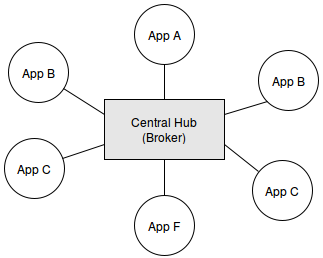
\includegraphics[width=0.4\textwidth]{images/central-hub.png}
    \caption{Mesh of multiple point-to-point connections}
    \label{fig:central-hub}
\end{figure}

%Hinweis: In der Literatur wird der hier genannte Broker oft in zwei
%verschiednen topoligien angeschaut: Bus und Broker, wobei der Broker lediglich
%für Transformation von Mesage zuständig ist. Die genaue Definition ist jedoch
%schwammig und unterscheided sich von Produkt und Hersteller. Deshalb fassen wir
%die Funktionalität von Bus und Broker zusammen zu Broker

\section{Message Broker in Detail}
\subsection{The Broker Pattern }
As the initial point for the detailed definition of a message broker we take the
\textit{Broker Pattern} of  \textit{Patterns of Software Architecture Volume 1}
which can be used to structure distributed systems with decoupled components.
Basically it distinguishes between two types of brokers, where the \textit{Direct
Broker} performs a initialization of a connection but the following communication
is only between the two endpoints. For messaging, the second variant,
\textit{Indirect Broker}, is a lot more interesting because it maintains all of
the communication between the nodes at every time. So let us define the message
broker as a refinement of the Indirect Broker Pattern for message-based
communication.\cite{POSA1} 

%\subsection{Structure}
The \textit{Broker Pattern} consists of five types of participating components,
which we can adapt for a message based environment by using the common terms.

\begin{description}
    \item[Producer (adapted from Client component)] \hfill \\
        {Applications that either generate data for later processing or
        access a service from another client in the messaging system. In both
        cases the producer pushes its messages to the broker and in general does
        not care about it anymore.}
    \item[Producer API (adapted from Client-Side-Proxy)] \hfill \\
        {Structural component which encapsulates messaging-specific
        functionality from the rest of the client code. Thereby, a call from the producer
        can be transformed to a message in the right format. The producer API
        directly communicates with the broker API.}
    \item[Broker] \hfill \\
        {Central component that acts as a mediator and is responsible for the
        transmission of messages from multiple producers to multiple consumers.
        A broker offers an API to the messaging clients, both for consumer and
        producer. It also must have kind of a directory for locating registered
        consumers.} 
    \item[Consumer (adapted from Server component)] \hfill \\
        {Basically the consumer is an endpoint which receives and processes a
            message for further activities. An \textit{Event Driven Consumer}
            handles incoming messages automatically as they are pushed from the
            broker. A \textit{Polling Consumer} explicitly gets messages when it
            wants to receive them from the broker. If a consumer provides a
            service to other clients, it also can act as a producer for sending
            back messages as response.}
    \item[Consumer API (adapted from Server Side Proxy)] \hfill \\
        {Structural component which encapsulates messaging-specific
        functionality from the rest of the client code. Based on incoming
        messages it calls services within the consumer component.}
\end{description}
\newpage
\subsection{Consumption Model}
A fundamental design decision of a message broker is whether consumers
    should pull data from brokers or brokers should push data to consumers. This
    has a direct impact on the performance of a broker system. In a
    push-based environment the consumers can be the bottleneck when its
    consumption rate falls below the rate of production. In a pull-based system,
    consumers which fall back can catch up at any time, the risk of
    bottleneck lies at the broker, thus a message broker should scale well.
\begin{figure}[H]
    \centering
     \begin{sequencediagram}
        %\newthread{broker}{Broker}
         \newinst[1]{producer}{Producer}
         \newinst[1]{producerProx}{Producer API}
         \newinst[1]{broker}{Broker}
        \newinst[1]{consumerProx}{Consumer API}
        \newinst[1]{consumer}{Consumer}
        \begin{messcall}
            {producer}{(1) Send Data}{producerProx}{}
        \end{messcall}
        \begin{call}
            {producerProx}{(2) Pack data to Message}{producerProx}{}
        \end{call}
        \begin{messcall}
            {producerProx}{(3) Transmit Message}{broker}{}
        \end{messcall}
        \begin{call}
            {broker}{(4) Write Message to internal Queue}{broker}{}
        \end{call}
        \begin{messcall}
            {broker}{(5) Deliver Message to single forward destination}{consumerProx}{} 
        \end{messcall}
        \begin{call}
            {consumerProx}{(6) Unpack Message}{consumerProx}{}
        \end{call}
        \begin{messcall}
            {consumerProx}{(7) Forward Data}{consumer}{}
        \end{messcall}
    \end{sequencediagram}
    \caption{Basic flow of a Broker event based consumption}
    \label{fig:MB-SSD-1}
\end{figure}
\newpage 
On the other hand, in a pull-based environment a consumer never knows whether a
message is ready for consumption or not. In the worst case this ends up with a read
loop where the consumer constantly needs to check the queue. \todo{more details}

\begin{figure}[H]
    \centering
     \begin{sequencediagram}
        %\newthread{broker}{Broker}
         \newinst[1]{producer}{Producer}
         \newinst[1]{producerProx}{Producer API}
         \newinst[1]{broker}{Broker}
        \newinst[1]{consumerProx}{Consumer API}
        \newinst[1]{consumer}{Consumer}
        \begin{messcall}
            {producer}{(1) Send Data}{producerProx}{}
        \end{messcall}
        \begin{call}
            {producerProx}{(2) Pack data to Message}{producerProx}{}
        \end{call}
        \begin{messcall}
            {producerProx}{(3) Transmit Message}{broker}{}
        \end{messcall}
        \begin{call}
            {broker}{(4) Write Message to internal Queue}{broker}{}
        \end{call}
        \begin{messcall}
            {consumer}{(5) Get Data}{consumerProx}{}
        \end{messcall}
        \begin{messcall}
            {consumerProx}{(6) Request Message}{broker}{} 
        \end{messcall}
        \begin{call}
            {broker}{(7) Get latest Message from internal Queue}{broker}{}
        \end{call}
        \begin{messcall}
            {broker}{(8) Deliver Message}{consumerProx}{} 
        \end{messcall}
        \begin{call}
            {consumerProx}{(9) Unpack Message}{consumerProx}{}
        \end{call}
        \begin{messcall}
            {consumerProx}{(10) Forward Data}{consumer}{}
        \end{messcall}
    \end{sequencediagram}
    \caption{Basic flow of a Broker with polling-based consumption}
    \label{fig:MB-SSD-1}
\end{figure}

%We saw that a \textit{Broker} acts like a mediator between to collaborating
%applications which do not need to know each other. The same does a message
%broker, of course in a message-oriented distributed system whereas the broker
%handles incoming messages from a source to a target and backwards.

%In such an environment it is essential that existing and new applications can be
%integrated into a single, coharent system at runtime. Often these applications
%are not speaking the same language and it need kind of a gateway for
%transforming messages into a format that can be unterstood by the receiver.
%\cite{TAN06}

%\subsection{Routing and Communicating}

%\subsection{Transformation}
%\subsection{Publish-Subscribe}
\subsection{Topic and Subscription Model}
\label{intro-messaging-publishsubscribe}
Message Broker systems are persisting incoming messages in an enhanced type of a
message queue, named topic. A topic allows the broker to deliver a message to
multiple independent consumers. Sending messages to the broker in the form of
publishing to a specific topic and on the other hand receiving messages only for
the specified topic, is called publish/subscribe. In contrast to a one-to-one
queue, the message broker requires the abilities to match messages on an
application-based level to act as a gateway for topic-related messages. Based on
the informations provided within the messages, the broker is able to
provide the messages to the client acting as a subscriber. In fact,
this publish/subscribe queue delivers a copy of the topic related messages to
the output channel. This also means that there can be more than one client that
consumes the topic-specific
messages and thus there can be more than one subscriber. Especially this feature
of having multiple consumers of a message channel, is decisive for using a
message broker in an environment where a distributed system processes the same stream of
data in multiple ways. \todo{ref to chapter}
\cite{EIP03} \cite{TAN06}

\begin{figure}[H]
    \centering
    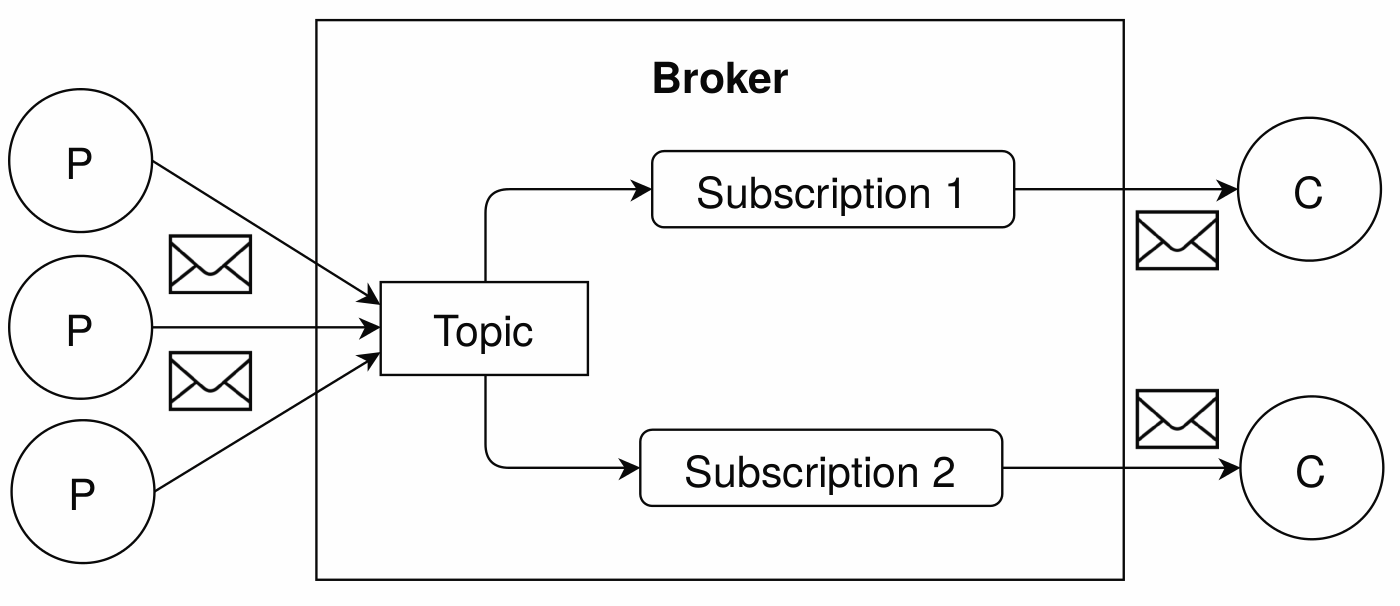
\includegraphics[width=0.7\textwidth]{images/topic-subscription.png}
    \caption{Broker forwards published messages to subscribers}
    \label{fig:topic-subscription}
\end{figure}

\subsection{Reliable Delivery}
    A reliable delivery of messages can promise a specific behaviour to producers
    and consumers. A message broker typically supports one ore more of the
    following guarantees.
    \textit{At most once} guarantees that messages may be lost but are never
    redelivered. \textit{At least once} defines that messages are never lost
    but may be redelivered. The \textit{Exactly once} semantic which is very
    typical guarantees that each message is delivered only once. Broker system
    which use the \textit{In Order} semantic deliver messages to the consumer in
    the strict same order in which they are sent from the producer to the broker. 

\section{Challenges of a Messaging System}
\todo[inline]{more details of cut off}
\label{intro-messaging-characteristics}
As described, a messaging system has its strengths in interoperability and loose
coupling of distributed computers. 
%Messaging löst also gewisse Schwierigkeiten von Distributed System bring aber
%selber neue Challenges auf: 
A message broker in turn has also many further
characteristics. The ones most related to our work are:

\begin{description}
    \item [Independence] \hfill \\
    {   The more independent a
        message broker is, the better it can be integrated in a existing
        environment. The use of standards and effective standardized interfaces
        promotes independence.}
        
    \item [Scalability] \hfill \\
    {    Ability to dynamically increase performance depending on work load. }
    \item [Latency]\hfill \\
    {    Time it takes to process a single message for consumption.  }
    \item [Fault Tolerance] \hfill \\
    {    Ability to recover after a failure with minimal message loss.
            Possibility to build redundancy through clustering and
            replication strategies such as master-slave or state machine
            replication. It is a significant characteristic how a
            message broker syncs its replications and elects which of the nodes
            to get active if the master fails. Also it is important that in case
            of failure the system can recover as quickly as possible and with
            minimal throughput deficit.   }
    \item [Persistency] \hfill \\ 
        {Ability to offer durable and persistent messages even if the broker
            systems restarts, crashes or consumer is inactive for a longer period of time
            (for instance batch processing systems). }
    \item [Throughput] \hfill \\
        {Proportion of messages which can be sent to a broker to the amount of
        messages which can be consumed in a fixed time interval.}
\end{description}


